\documentclass{standalone}
\usepackage{tikz}
\usetikzlibrary{patterns, positioning}

\begin{document}
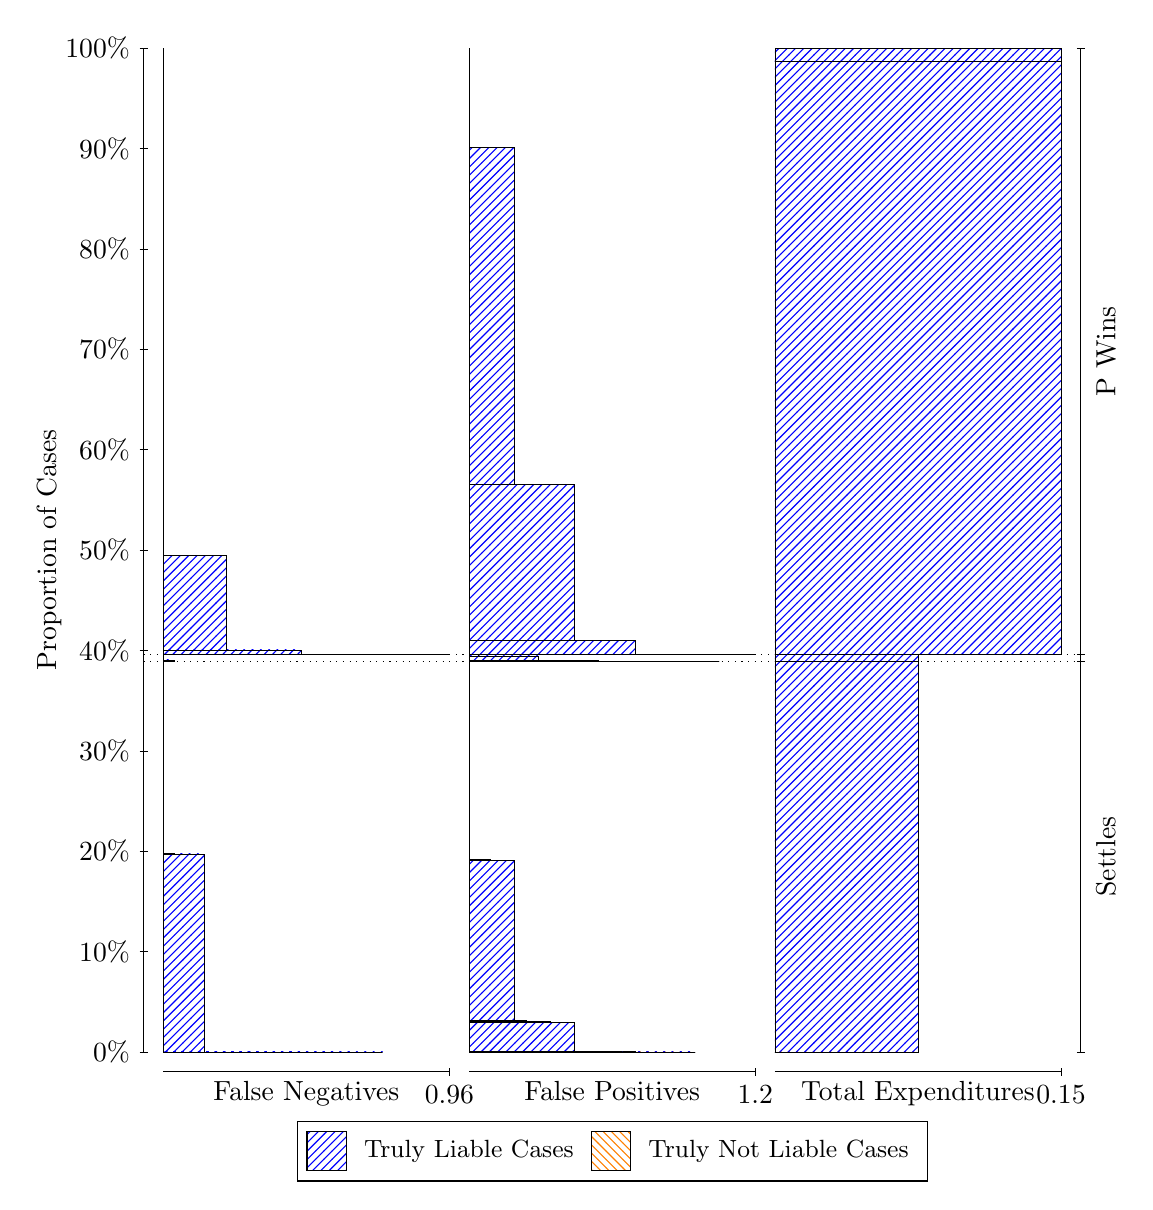
\begin{tikzpicture}
\draw[black, very thin] (1.5,1.75) -- (1.5,14.5);
\node[rotate=90, anchor=center] at (0.3, 8.125) {Proportion of Cases};
\draw[black, very thin] (1.45,1.75) -- (1.55,1.75);
\node[anchor=east] at (1.45, 1.75) {0\%};
\draw[black, very thin] (1.45,3.025) -- (1.55,3.025);
\node[anchor=east] at (1.45, 3.025) {10\%};
\draw[black, very thin] (1.45,4.3) -- (1.55,4.3);
\node[anchor=east] at (1.45, 4.3) {20\%};
\draw[black, very thin] (1.45,5.575) -- (1.55,5.575);
\node[anchor=east] at (1.45, 5.575) {30\%};
\draw[black, very thin] (1.45,6.85) -- (1.55,6.85);
\node[anchor=east] at (1.45, 6.85) {40\%};
\draw[black, very thin] (1.45,8.125) -- (1.55,8.125);
\node[anchor=east] at (1.45, 8.125) {50\%};
\draw[black, very thin] (1.45,9.4) -- (1.55,9.4);
\node[anchor=east] at (1.45, 9.4) {60\%};
\draw[black, very thin] (1.45,10.675) -- (1.55,10.675);
\node[anchor=east] at (1.45, 10.675) {70\%};
\draw[black, very thin] (1.45,11.95) -- (1.55,11.95);
\node[anchor=east] at (1.45, 11.95) {80\%};
\draw[black, very thin] (1.45,13.225) -- (1.55,13.225);
\node[anchor=east] at (1.45, 13.225) {90\%};
\draw[black, very thin] (1.45,14.5) -- (1.55,14.5);
\node[anchor=east] at (1.45, 14.5) {100\%};

\draw[black, very thin] (13.4,1.75) -- (13.4,14.5);
\draw[black, very thin] (13.35,1.75) -- (13.45,1.75);
\node[anchor=west] at (13.35, 1.75) {};
\draw[black, very thin] (13.35,6.7131) -- (13.45,6.7131);
\node[anchor=west] at (13.35, 6.7131) {};
\draw[black, very thin] (13.35,6.7966) -- (13.45,6.7966);
\node[anchor=west] at (13.35, 6.7966) {};
\draw[black, very thin] (13.35,14.5) -- (13.45,14.5);
\node[anchor=west] at (13.35, 14.5) {};

\draw[black, very thin, pattern color=blue, pattern=north east lines] (1.75,1.75) rectangle (4.534,1.75);
\draw[black, very thin, pattern color=blue, pattern=north east lines] (1.75,1.75) rectangle (4.1565,1.75);
\draw[black, very thin, pattern color=blue, pattern=north east lines] (1.75,1.75) rectangle (3.779,1.75);
\draw[black, very thin, pattern color=blue, pattern=north east lines] (1.75,1.75) rectangle (3.5903,1.75);
\draw[black, very thin, pattern color=blue, pattern=north east lines] (1.75,1.75) rectangle (3.4015,1.75);
\draw[black, very thin, pattern color=blue, pattern=north east lines] (1.75,1.75) rectangle (3.2128,1.75);
\draw[black, very thin, pattern color=blue, pattern=north east lines] (1.75,1.75) rectangle (3.024,1.75);
\draw[black, very thin, pattern color=blue, pattern=north east lines] (1.75,1.75) rectangle (2.8353,1.75);
\draw[black, very thin, pattern color=blue, pattern=north east lines] (1.75,1.75) rectangle (2.6465,1.7502);
\draw[black, very thin, pattern color=blue, pattern=north east lines] (1.75,1.7502) rectangle (2.6465,1.7502);
\draw[black, very thin, pattern color=blue, pattern=north east lines] (1.75,1.7502) rectangle (2.4578,1.7502);
\draw[black, very thin, pattern color=blue, pattern=north east lines] (1.75,1.7502) rectangle (2.269,4.2657);
\draw[black, very thin, pattern color=blue, pattern=north east lines] (1.75,4.2657) rectangle (2.0803,4.2661);
\draw[black, very thin, pattern color=blue, pattern=north east lines] (1.75,4.2661) rectangle (1.8916,4.2704);
\draw[black, very thin, pattern color=orange, pattern=north west lines] (1.75,4.2704) rectangle (1.75,4.2704);
\draw[black, very thin, pattern color=blue, pattern=north east lines] (1.75,4.2704) rectangle (1.75,6.7131);
\draw[black, very thin, pattern color=blue, pattern=north east lines] (1.75,6.7131) rectangle (1.8916,6.7283);
\draw[black, very thin, pattern color=orange, pattern=north west lines] (1.75,6.7283) rectangle (1.75,6.7283);
\draw[black, very thin, pattern color=blue, pattern=north east lines] (1.75,6.7283) rectangle (1.75,6.7966);
\draw[black, very thin, pattern color=blue, pattern=north east lines] (1.75,6.7966) rectangle (5.3833,6.7966);
\draw[black, very thin, pattern color=blue, pattern=north east lines] (1.75,6.7966) rectangle (4.4396,6.7968);
\draw[black, very thin, pattern color=blue, pattern=north east lines] (1.75,6.7968) rectangle (3.4959,6.856);
\draw[black, very thin, pattern color=blue, pattern=north east lines] (1.75,6.856) rectangle (2.5522,8.0601);
\draw[black, very thin, pattern color=orange, pattern=north west lines] (1.75,8.0601) rectangle (1.75,8.0601);
\draw[black, very thin, pattern color=blue, pattern=north east lines] (1.75,8.0601) rectangle (1.75,14.5);
\draw[black, very thin, pattern color=orange, pattern=north west lines] (5.6333,1.75) rectangle (8.5018,1.75);
\draw[black, very thin, pattern color=blue, pattern=north east lines] (5.6333,1.75) rectangle (8.5018,1.75);
\draw[black, very thin, pattern color=orange, pattern=north west lines] (5.6333,1.75) rectangle (8.1958,1.75);
\draw[black, very thin, pattern color=blue, pattern=north east lines] (5.6333,1.75) rectangle (8.1958,1.75);
\draw[black, very thin, pattern color=orange, pattern=north west lines] (5.6333,1.75) rectangle (7.8898,1.75);
\draw[black, very thin, pattern color=blue, pattern=north east lines] (5.6333,1.75) rectangle (7.8898,1.75);
\draw[black, very thin, pattern color=blue, pattern=north east lines] (5.6333,1.75) rectangle (7.7368,1.7528);
\draw[black, very thin, pattern color=orange, pattern=north west lines] (5.6333,1.7528) rectangle (7.5839,1.7528);
\draw[black, very thin, pattern color=blue, pattern=north east lines] (5.6333,1.7528) rectangle (7.5839,1.7528);
\draw[black, very thin, pattern color=blue, pattern=north east lines] (5.6333,1.7528) rectangle (7.4309,1.7528);
\draw[black, very thin, pattern color=orange, pattern=north west lines] (5.6333,1.7528) rectangle (7.2779,1.7528);
\draw[black, very thin, pattern color=blue, pattern=north east lines] (5.6333,1.7528) rectangle (7.2779,1.7529);
\draw[black, very thin, pattern color=blue, pattern=north east lines] (5.6333,1.7529) rectangle (7.1249,1.7532);
\draw[black, very thin, pattern color=orange, pattern=north west lines] (5.6333,1.7532) rectangle (6.9719,1.7532);
\draw[black, very thin, pattern color=blue, pattern=north east lines] (5.6333,1.7532) rectangle (6.9719,2.1247);
\draw[black, very thin, pattern color=blue, pattern=north east lines] (5.6333,2.1247) rectangle (6.8189,2.1248);
\draw[black, very thin, pattern color=blue, pattern=north east lines] (5.6333,2.1248) rectangle (6.666,2.1248);
\draw[black, very thin, pattern color=orange, pattern=north west lines] (5.6333,2.1248) rectangle (6.666,2.1248);
\draw[black, very thin, pattern color=blue, pattern=north east lines] (5.6333,2.1248) rectangle (6.666,2.1343);
\draw[black, very thin, pattern color=blue, pattern=north east lines] (5.6333,2.1343) rectangle (6.513,2.1392);
\draw[black, very thin, pattern color=blue, pattern=north east lines] (5.6333,2.1392) rectangle (6.36,2.1467);
\draw[black, very thin, pattern color=blue, pattern=north east lines] (5.6333,2.1467) rectangle (6.207,4.1815);
\draw[black, very thin, pattern color=blue, pattern=north east lines] (5.6333,4.1815) rectangle (6.054,4.1817);
\draw[black, very thin, pattern color=blue, pattern=north east lines] (5.6333,4.1817) rectangle (5.9011,4.1817);
\draw[black, very thin, pattern color=blue, pattern=north east lines] (5.6333,4.1817) rectangle (5.9011,4.1927);
\draw[black, very thin, pattern color=blue, pattern=north east lines] (5.6333,4.1927) rectangle (5.7481,4.1971);
\draw[black, very thin, pattern color=blue, pattern=north east lines] (5.6333,4.1971) rectangle (5.6333,6.7131);
\draw[black, very thin, pattern color=orange, pattern=north west lines] (5.6333,6.7131) rectangle (8.8077,6.7131);
\draw[black, very thin, pattern color=blue, pattern=north east lines] (5.6333,6.7131) rectangle (8.8077,6.7131);
\draw[black, very thin, pattern color=blue, pattern=north east lines] (5.6333,6.7131) rectangle (8.0428,6.7132);
\draw[black, very thin, pattern color=blue, pattern=north east lines] (5.6333,6.7132) rectangle (7.2779,6.7259);
\draw[black, very thin, pattern color=blue, pattern=north east lines] (5.6333,6.7259) rectangle (6.513,6.7814);
\draw[black, very thin, pattern color=blue, pattern=north east lines] (5.6333,6.7814) rectangle (5.7481,6.7966);
\draw[black, very thin, pattern color=orange, pattern=north west lines] (5.6333,6.7966) rectangle (9.2667,6.7966);
\draw[black, very thin, pattern color=blue, pattern=north east lines] (5.6333,6.7966) rectangle (9.2667,6.7966);
\draw[black, very thin, pattern color=orange, pattern=north west lines] (5.6333,6.7966) rectangle (8.5018,6.7966);
\draw[black, very thin, pattern color=blue, pattern=north east lines] (5.6333,6.7966) rectangle (8.5018,6.7992);
\draw[black, very thin, pattern color=orange, pattern=north west lines] (5.6333,6.7992) rectangle (7.7368,6.7992);
\draw[black, very thin, pattern color=blue, pattern=north east lines] (5.6333,6.7992) rectangle (7.7368,6.9809);
\draw[black, very thin, pattern color=orange, pattern=north west lines] (5.6333,6.9809) rectangle (6.9719,6.9809);
\draw[black, very thin, pattern color=blue, pattern=north east lines] (5.6333,6.9809) rectangle (6.9719,8.9598);
\draw[black, very thin, pattern color=orange, pattern=north west lines] (5.6333,8.9598) rectangle (6.207,8.9598);
\draw[black, very thin, pattern color=blue, pattern=north east lines] (5.6333,8.9598) rectangle (6.207,13.237);
\draw[black, very thin, pattern color=blue, pattern=north east lines] (5.6333,13.237) rectangle (5.6333,14.5);
\draw[black, very thin, pattern color=orange, pattern=north west lines] (9.5167,1.75) rectangle (11.333,1.75);
\draw[black, very thin, pattern color=blue, pattern=north east lines] (9.5167,1.75) rectangle (11.333,6.7131);
\draw[black, very thin, pattern color=orange, pattern=north west lines] (9.5167,6.7131) rectangle (11.333,6.7131);
\draw[black, very thin, pattern color=blue, pattern=north east lines] (9.5167,6.7131) rectangle (11.333,6.7966);
\draw[black, very thin, pattern color=orange, pattern=north west lines] (9.5167,6.7966) rectangle (13.15,6.7966);
\draw[black, very thin, pattern color=blue, pattern=north east lines] (9.5167,6.7966) rectangle (13.15,14.33);
\draw[black, very thin, pattern color=orange, pattern=north west lines] (9.5167,14.33) rectangle (13.15,14.33);
\draw[black, very thin, pattern color=blue, pattern=north east lines] (9.5167,14.33) rectangle (13.15,14.5);
\draw[black, dotted] (1.5,6.7131) -- (13.4,6.7131);
\draw[black, dotted] (1.5,6.7966) -- (13.4,6.7966);
\draw[black, very thin] (1.75,1.5) -- (5.3833,1.5);
\node[anchor=north] at (3.5667, 1.5) {False Negatives};
\draw[black, very thin] (5.3833,1.45) -- (5.3833,1.55);
\node[anchor=north] at (5.3833, 1.45) {0.96};

\draw[black, very thin] (5.6333,1.5) -- (9.2667,1.5);
\node[anchor=north] at (7.45, 1.5) {False Positives};
\draw[black, very thin] (9.2667,1.45) -- (9.2667,1.55);
\node[anchor=north] at (9.2667, 1.45) {1.2};

\draw[black, very thin] (9.5167,1.5) -- (13.15,1.5);
\node[anchor=north] at (11.333, 1.5) {Total Expenditures};
\draw[black, very thin] (13.15,1.45) -- (13.15,1.55);
\node[anchor=north] at (13.15, 1.45) {0.15};

\node[black, centered, rotate=90] at (13.72, 4.2316) {Settles};

\node[black, centered, rotate=90] at (13.72, 10.648) {P Wins};

\draw (7.449999999999999,1.5) node[draw=none] (baseCoordinate) {};
\begin{scope}[align=center]
        \matrix[scale=0.5, draw=black, below=0.5cm of baseCoordinate, nodes={draw}, column sep=0.1cm]{
            \node[rectangle, draw, minimum width=0.5cm, minimum height=0.5cm, pattern=north east lines, pattern color=blue] {}; &
            \node[draw=none, font=\small] (B) {Truly Liable Cases}; &
            \node[rectangle, draw, minimum width=0.5cm, minimum height=0.5cm, pattern=north west lines, pattern color=orange] {}; &
            \node[draw=none, font=\small] (B) {Truly Not Liable Cases}; \\
            };
\end{scope}

\end{tikzpicture}
\end{document}